\documentclass[11pt,a4paper]{report}
\usepackage[utf8]{inputenc}
\usepackage[french]{babel}
\usepackage[T1]{fontenc}
\usepackage{amsmath}
\usepackage{amsfonts}
\usepackage{amssymb}
\usepackage{xcolor}
\usepackage{gensymb}

\usepackage{geometry}
\geometry{hmargin=2.5cm,vmargin=1.5cm}
\usepackage{wasysym}
\usepackage{graphicx}

\author{Mathieu Sarrat}
\title{LC14 - Détermination de constantes d'équilibre}

\makeatletter
\renewcommand{\thesection}{\@arabic\c@section}
\makeatother


\begin{document}
\maketitle

\section*{Niveau, Pré-requis et objectifs}
\begin{itemize}
	\item \textbf{Niveau :} MPSI\\
	
	\item \textbf{Pré-requis :}
	\begin{itemize}
		\item Titrages\\
	\end{itemize}
	
	\item \textbf{Objectifs :}
	\begin{itemize}
		\item Mesurer des constantes d'équilibre avec des méthodes diverses.\\
	\end{itemize}
		
	\item \textbf{Matériel :}
	\begin{itemize}
		\item Thermomètre\\
		
		\item pH-mètre et solutions d'étalonnage,
		\item Solution titrée d'acide éthanoïque à $1.00 \times 10^{-1}$ mol/L,
		\item Solution titrée d'éthanoate de sodium à $1.00 \times 10^{-1}$ mol/L,
		\item Solution titrée de soude à $1.00 \times 10^{-1}$ mol/L.\\
		
		\item Conductimètre et solutions d'étalonnage,
		\item Sulfate de calcium solide,
		\item Montage de filtration sous vide.\\

		\item 50 mL de solution de nitrate d'argent à $C_1 = 0.050$ mol/L
		\item 100 mL de solution de thiocyanate de potassium à $C_2 = 0.070$ mol/L
		\item électrode au sulfate mercureux ($E_\text{ref} = 0.6125 V$)
		\item électrode d'argent ($E\degree(\text{Ag}^+/\text{Ag}_\text{(s)}) =$ 0.79 V ) 
		et matériel de nettoyage\\

		\item Solution titrée d'acide benzoïque ($\sim 10^-2$ mol/L),
		\item Solution titrée de soude à (adapter à celle d'acide benzoïque).
		\item BBT
	\end{itemize}
		
	\item \textbf{Recommandations :}
	\begin{itemize}
		\item Relever la température pour chaque expérience, puisqu'une constante d'équilibre dépend 			de la température.
		\item Dissoudre le sulfate de calcium avant la leçon, assez tôt dans la préparation, et 					laisser l'agitation en fonctionnement jusqu'à faire la mesure.
	\end{itemize}
\end{itemize}

\newpage
\section*{Introduction}

Nous avons introduit, dans une leçon précédente, la notion de constante d'équilibre. Cette quantité, fonction de la température, caractérise un équilibre chimique donné. On peut relier la valeur de la constante d'équilibre aux activités chimiques des constituants présents dans le milieu réactionnel lorsque l'équilibre est effectivement atteint. C'est la loi d'action de masse (ou loi de Guldberg et Waage) :
\begin{equation}
	K\degree(T) = \Pi_{i}\left( \text{a}_i^{\nu_i} \right),
\end{equation}
où $\nu_i$ est le coefficient stœchiométrique algébrique (positif pour un produit, négatif pour un réactif) du réactif/produit i et où $\text{a}_i$ désigne son activité chimique.\\

L'objectif de cette leçon est de mettre en œuvre plusieurs approches expérimentales pour déterminer la valeur de ces constantes. Nous nous appuierons sur des exemples précis.

\section{Mesure d'une constante d'acidité}\label{sec:1}

\subsection{Constante d'acidité de l'acide éthanoïque}

On veut déterminer la constante d'acidité du couple $\text{CH}_3\text{COOH}/\text{CH}_3\text{COO}^-$, constante d'équilibre de la réaction de dissociation de l'acide dans l'eau :
\begin{equation}
	\boxed{\text{CH}_3\text{COOH}_\text{(aq)} + \text{H}_2\text{O}_\text{(l)} 
	= {\text{CH}_3\text{COO}^-}_\text{(aq)} + {\text{H}_3\text{O}^+}_\text{(aq)}}. 
\end{equation}
Elle a pour expression
\begin{equation}
	K_A \equiv 
	\frac{a({\text{CH}_3\text{COO}^-}_\text{(aq)})\;a({\text{H}_3\text{O}^+}_\text{(aq)})}
	{a(\text{CH}_3\text{COOH}_\text{(aq)})\;a(\text{H}_2\text{O}_\text{(l)})}
\end{equation}
où les activités sont calculées \textbf{à l'équilibre}, 
et si la solution est suffisamment diluée ($c < 1.0\times 10^{-1}$ mol/L),
\begin{equation}
	a_\text{solvant} = 1\quad\text{et}\quad a_\text{soluté} = \frac{[\text{soluté}]}{c\degree}, 
\end{equation}
les concentrations étant données en mol/L et $c\degree =$ 1 mol/L.\\

D'où
\begin{equation}
	\boxed{K_A = \frac{[{\text{CH}_3\text{COO}^-}]_\text{eq}[{\text{H}_3\text{O}^+}]_\text{eq}}
	{[\text{CH}_3\text{COOH}]_\text{eq}}}.
\end{equation}

\subsection{Mélange d'un acide faible et de sa base conjuguée}
\textcolor{red}{Le Maréchal, Chimie Générale (Tome 1), p9}.\\

Étalonner le pH-mètre en utilisant des solutions tampon à pH $=$ 4 et pH $=$ 7.

\subsubsection{Principe :}
On mélange en proportions connues des solutions d'acide acétique et d'éthanoate de sodium de mêmes concentrations ($1.0\times10^{-1}$\;mol/L) et on relève le pH au pH-mètre.\\

Dresser un tableau d'avancement littéral. Comme on a un acide et une base faibles, on suppose qu'il va peu se dissocier : on calcule donc les concentrations à l'équilibre connaissant les concentrations initiales et les volumes introduits.\\

On passe au logarithme décimal l'expression de $K_A$ en fonction des concentrations et on trace 
\begin{equation}
	\text{pH} = f\left(\text{log}_{10}\left(\frac{[\text{A}^-]}{[\text{AH}]}\right)\right)
	= \text{pK}_\text{A} + \text{log}_{10}\left(\frac{[\text{A}^-]}{[\text{AH}]}\right).
\end{equation}

L'ordonnée à l'origine permet de remonter au $\text{pK}_\text{A}$ et on en déduit la constante d'acidité. On vérifie que le mélange équimolaire donne un pH égal au pKa, sans quoi il y a un souci avec le pH-mètre (ou alors les solutions ne sont pas assez diluées ou trop diluées).

\subsection{Mesure par titrage à la demi-équivalence}
\textcolor{red}{Cachau-Hereillat, Acide-Base, p137}.

\subsubsection{Principe :}
On remarque qu'en réalisant un mélange équimolaire entre un acide faible et sa base conjuguée, le pH mesuré correspond au $\text{pK}_\text{A}$ du couple. Lors d'un dosage par une base forte, on consomme l'acide faible pour produire sa base conjuguée.\\

\`A demi-équivalence, c'est à dire lorsque la moitié du réactif titré a été consommée et que la solution d'acide n'est pas trop diluée, on a
\begin{equation}
	[\text{A}^-] = [\text{AH}] \quad\text{et donc}\quad \text{pH} = \text{pK}_\text{A}.
\end{equation} 

Nous allons suivre le dosage de l'acide acétique par la soude à l'aide d'un pH-mètre. La réaction de dosage est la suivante
\begin{equation}
	\boxed{\text{CH}_3\text{COOH}_\text{(aq)} + \text{HO}^-_\text{(aq)} 
	\longrightarrow \text{H}_2\text{O}_\text{(l)} + {\text{CH}_3\text{COO}^-}_\text{(aq)}}.
\end{equation}

\subsubsection{Matériel et protocole :}
\begin{itemize}
	\item Solution de soude titrée à $1.00 \times 10^{-1}$ mol/L
	\item Solution $\mathcal{S}_0$ d'acide éthanoïque à $1.00 \times 10^{-1}$ mol/L.\\
	
	\item Préparer une solution d'acide à $1.00 \times 10^{-2}$ mol/L de 100 mL : 10 mL d'acide 				éthanoïque $\mathcal{S}_0$ et 90 mL d'eau distillée.
	\item Doser par la soude, contenue dans la burette, 
		faire l'acquisition du pH et du volume versé.
	\item Traitement sur Regressi : tracer la dérivée pour mesurer le volume équivalent, puis la 				demi-équivalence. Lire le pH pour ce volume, en déduire le $\text{pK}_\text{A}$.
\end{itemize}

\subsubsection{Remarque :}
Si l'acide est trop dilué, c'est à dire que sa dissociation est déjà importante, on va doser moins d'acide, donc fausser la mesure. Le pH de la solution initiale risque d'être déjà supérieur au 
$\text{pK}_\text{A}$.

\newpage
\section{Mesure d'un produit de solubilité}\label{sec:2}

\subsection{Produit de solubilité du sulfate de calcium par conductimétrie}
\textcolor{red}{Par conductimétrie : Le Maréchal Chimie Générale, p160}\\

Dans le cas d'un solide peu soluble, la méthode par titrage est trop imprécise et on a recours à d'autres méthodes, par exemple la conductimétrie lorsqu'on a affaire à un solide ionique (en se dissolvant, il libère des ions).\\

On se propose de déterminer le produit de solubilité $\text{K}_s$ du sulfate de calcium dans l'eau \textcolor{blue}{(relever la température)}. L'équation de dissolution du solide est la suivante :
\begin{equation}
	\text{CaSO}_{4,\text{(s)}} \rightleftarrows \text{Ca}^{2+} + \text{SO}_4^{2-}.
\end{equation}
Lorsque le solide existe, on finit par atteindre un équilibre de solubilité. L'activité du solide, seul dans sa phase, est de 1. On approxime celle des ions par le rapport de leur concentration sur la concentration standard, d'où l'expression du produit de solubilité :
\begin{equation}
	\boxed{\text{K}_s(T) = [\text{Ca}^{2+}]_\text{eq} [{\text{SO}_4}^{2-}]_\text{eq}}
\end{equation}
\textbf{Cette relation n'est satisfaite que si le solide existe dans le milieu réactionnel.}

\subsubsection{En préparation :}

\begin{itemize}
	\item Étalonner le conductimètre
	\item Mesurer la conductance G de l'eau distillée (attention, les concentrations sont 
		en $mol/m^{-3}$ dans les calculs.
	\item Dans un bécher de 100 mL d'eau distillée, on introduit une spatule de sulfate de calcium 			solide (tout ne doit pas se dissoudre). Introduire un barreau aimanté et agiter. Ne pas 				interrompre l'agitation jusqu'au moment de faire une mesure. On peut aussi filtrer la solution 			pour éliminer le solide.
\end{itemize}

\subsubsection{En direct, mesure et exploitation :}	
\begin{itemize}
	\item Mesurer la conductance G de la solution de sulfate de calcium, retrancher la conductance 				de l'eau distillée.
	\item  $\sigma = G L/S$ (avec S/L $=$ 1 cm normalement, pas forcément besoin avec étalonnage)\\
	\item \textcolor{blue}{Loi de Kolhrausch :}
	\begin{equation}
		\sigma = \lambda^o(\text{Ca}^{2+})[\text{Ca}^{2+}]_\text{eq} 
		+ \lambda^o({\text{SO}_4}^{2-})[{\text{SO}_4}^{2-}]_\text{eq},
	\end{equation}
	or les concentrations sont égales, et on connaît les conductivités molaires ioniques limite
	$\lambda^o(\text{Ca}^{2+}) = 11,9\;S.\text{m}^2\text{mol}^{-1}$ 
	et $\lambda^o({\text{SO}_4}^{2-}) = 16.0\;S.\text{m}^2\text{mol}^{-1}$.\\
	
	\item La valeur tabulée pour 25\degree C est $K_s = 2.4\times10^{-5}$.
\end{itemize}

\newpage
\subsection{Produit de solubilité du thiocyanate d'argent par potentiométrie}
\textcolor{red}{Daumarie, Florilège de chimie pratique, p117}\\

On veut déterminer le $K_s$ du thiocyanate d'argent AgSCN à 25\degree C (valeur tabulée : pKs $=$ 12). On procède par titrage potentiométrique en dosant une solution de nitrate d'argent par une solution titrée de thiocyanate de potassium (KSCN).\\

\subsubsection*{Matériel et protocole}
\begin{itemize}
	\item 50 mL de solution de nitrate d'argent à $C_1 = 0.050$ mol/L
	\item 100 mL de solution de thiocyanate de potassium à $C_2 = 0.070$ mol/L
	\item électrode au sulfate mercureux ($E_\text{ref} = 0.6125 V$)
	\item électrode d'argent ($E\degree(\text{Ag}^+/\text{Ag}_\text{(s)}) =$ 0.79 V ) 
		et matériel de nettoyage
\end{itemize}

\begin{itemize}
	\item Nettoyer l'électrode d'argent pour retirer l'oxyde, rincer à l'eau distillée abondamment, 				sécher,
	\item Remplir la burette avec la solution de thiocyanate de potassium;
	\item Prélever $V_1 =$ 10 mL de solution de nitrate d'argent et introduire dans un bécher;
	\item Ajouter \textbf{précisément} $V_\text{eau} =$ 50 mL d'eau distillée dans le bécher (cf. seconde mesure);
	\item Connecter les électrodes à un voltmètre, les plonger dans le bécher;
	\item Relever la différence de potentiel $\Delta E$ en fonction du volume de solution titrante versé;
	\item Tracer la dérivée, si besoin, pour mesurer le volume équivalent.
	
\end{itemize}
\subsubsection*{Exploitation}
La réaction de titrage est la suivante
\begin{equation}
	\boxed{\text{Ag}^+ + \text{SCN}^- \rightleftarrows \text{AgSCN}_\text{(s)}},\;
	\text{de constante d'équilibre} K\degree(T) = \frac{1}{K_s} = \frac{1}{[\text{Ag}^+]_\text{eq}				[\text{SCN}^-]_\text{eq}}.
\end{equation}

	\begin{figure}[h!]
		\begin{center}
			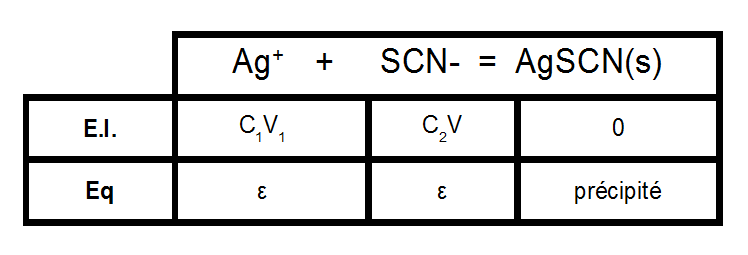
\includegraphics[scale = 0.4]{AgSCN.png}
		\end{center}
		\caption{Tableau d'avancement de la réaction de dosage. 
		$E\degree(\text{Ag}^+/\text{Ag}_\text{(s)}) =$ 0.79 V. }
	\end{figure}
	
\`A l'équivalence du dosage $C_1 V_1 = C_2 V_\text{eq}$ avec $V_\text{eq} = 7.14$ mL prévu, et après réaction, l'équilibre de solubilité sera réalisé d'où
\begin{equation}
	K_s = \epsilon^2 \quad\text{d'où}\quad [\text{Ag}^+] = \epsilon = \sqrt{K_s}.
\end{equation}
\`A l'équilibre et à 25\degree C, le potentiel est donné par la loi de Nernst
\begin{equation}
	E(\text{Ag}^+/\text{Ag}_\text{(s)}) 
	= E\degree(\text{Ag}^+/\text{Ag}_\text{(s)}) + 0.06\;\text{log}\;[\text{Ag}^+],
\end{equation}
donc à l'équivalence on aura
\begin{equation}
	\Delta E = E\degree(\text{Ag}^+/\text{Ag}_\text{(s)}) - E_\text{ref} + 0.03\;\text{log}\;K_s.
\end{equation}

On peut aussi faire une mesure en se plaçant en large excès de thiocyanate (V $= 2V_\text{eq}$), de sorte qu'une erreur sur la lecture du volume ait moins d'impact qu'à l'équivalence où la différence de potentiel décroît brutalement, avec une pente quasi verticale :
\begin{equation}
	[\text{SCN}^-] = \frac{C_2V-C_1V_1}{V_\text{tot}+ V}\quad\text{avec}\quad V_\text{tot} 
	= V_1 + V_\text{eau},
\end{equation}
et on aura $[\text{Ag}^+] = K_s/[\text{SCN}^-]$ à injecter dans la relation de Nernst.

\newpage
\section{Mesure d'un coefficient de partage}\label{sec:3}

\subsection{Définition et principe de l'expérience}

L'opération d'extraction liquide-liquide est une technique largement utilisée en chimie.
Elle intervient en général à la fin d'une synthèse pour traiter un brut réactionnel liquide,
c'est à dire un mélange qui contient le produit de la réaction, les produits secondaires, les réactifs en excès et le solvant. Le but est d'isoler le produit d'intérêt solvaté initialement dans un solvant S en le faisant passer dans une phase organique ou aqueuse (solvant S' : on fait passer la substance d'un solvant à un autre. L'extraction n'est possible que si les deux liquides ne sont pas miscibles. Bien entendu, le produit d'intérêt doit avoir la meilleure différence possible d'affinité entre les deux solvants.

\subsubsection{En préparation :}
\textcolor{blue}{L'extraction n'est pas au programme et doit avoir été faite en préparation, de même que la séparation des deux phases : on explique seulement son principe, on donne les quantités utilisées puis on passe au dosage de la phase aqueuse.}\\

\begin{itemize}
	\item Acide benzoïque (s $=$ 2.9 g/L à 25$\degree$ C dans l'eau, M $=$ 122.1 g/mol,
		 pKa $=$ 4.2) : préparer 200 mL de solution saturée $S_0$ (ou utiliser une solution déjà 				 prête, \textbf{de concentration titrée})
	\item Extraction d'un volume de $V_0 =$ 50 mL de la solution $S_0$ par $V_1 =$ 25 mL d'huile de 					tournesol avec ampoule à décanter. Récupération des deux phases, dans deux béchers.
	\begin{figure}[h!]
		\begin{center}
			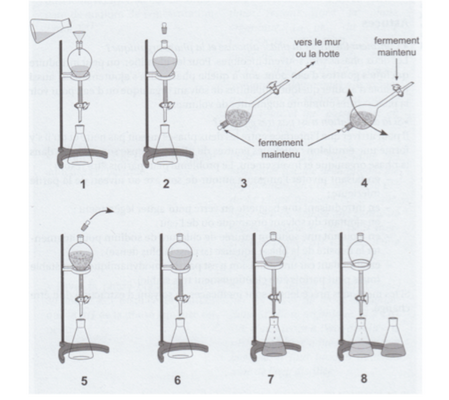
\includegraphics[scale = 1]{ampoule.png}
		\end{center}
		\caption{Protocole pour l'extraction liquide-liquide suivie de la décantation.}
	\end{figure}
\end{itemize}

On a réalisé en préparation l'extraction de l'acide benzoïque d'une solution aqueuse par un volume d'huile de tournesol. L'équilibre de partage entre les deux phases est réalisé, et la concentration en acide benzoïque de chaque phase vérifie 
\begin{equation}
	\boxed{K\degree (T) = \frac{[\text{PhCOOH}]_\text{orga}}{[\text{PhCOOH}]_\text{eau}}.}
\end{equation}
où K\degree(T) désigne le coefficient de partage (constante thermodynamique de l'équilibre de partage).

\subsection{Mesure par titrage colorimétrique}

Nous nous proposons de réaliser la détermination de K\degree \textcolor{blue}{(relever la température)}.

\subsubsection*{Dosage}

On fait un dosage colorimétrique de la phase aqueuse par la soude de concentration $C_T$, en utilisant le BBT comme indicateur coloré. Pipeter $\text{V}_p = 10$ mL de phase aqueuse doser en appuyant le bout de la pipette contre le fond du bécher, pour éviter de récupérer d'éventuels restes de la phase organique qui surnageraient. Introduire le prélèvement dans un erlenmeyer de volume adapté, ainsi qu'un agitateur magnétique. Verser quelques gouttes de BBT.

La réaction de titrage est la suivante :
\begin{equation}
	\text{\text{PhCOOH}} + \text{HO}^- \longrightarrow \text{PhCOO}^- + \text{H}_2\text{O}
\end{equation}

L'équivalence est atteinte lorsque le BBT vire au bleu. On relève le volume équivalent $V_\text{eq}$, puis on calcule les concentrations dans les deux phases.

\subsubsection*{Exploitation :}
\begin{itemize}
	\item \textcolor{blue}{Calcul de la concentration d'acide en phase aqueuse :}
	\begin{equation}
		\boxed{[\text{PhCOOH}]_\text{eau} = \frac{C_T\;V_\text{eq}}{\text{V}_p}},
	\end{equation}
		
	\item \textcolor{blue}{Calcul de la concentration d'acide en phase organique : }
		\begin{itemize}
			\item on calcule la quantité de matière présente dans la \textbf{totalité} de la phase 						aqueuse (on connait le volume de solution $\mathcal{S}_0$, qui est par définition le 				volume de la phase aqueuse)
				\begin{equation}
					n(\text{eau}) = [\text{PhCOOH}]_\text{eau}\;V_0,
				\end{equation}
			\item on calcule la quantité de matière totale d'acide benzoïque
				\begin{equation}
					n(\text{tot}) = \text{C}_0\;\text{V}_0
				\end{equation}
			\item d'où la concentration d'acide en phase organique
				\begin{equation}
					[\text{PhCOOH}]_\text{orga} = \frac{n(\text{tot}) - n(\text{eau})}{\text{V}_1}
				\end{equation}								  
		\end{itemize}
	\item \textcolor{blue}{Calcul de la constante de partage :}
		\begin{equation}
			K\degree (T) = \frac{[\text{PhCOOH}]_\text{orga}}{[\text{PhCOOH}]_\text{eau}}.
		\end{equation}
\end{itemize}


\newpage
\section*{Conclusion}

Nous avons mesuré des constantes d'équilibre. En seconde année, vous verrez comment calculer ces grandeurs, à partir de lois découlant des principes de la thermodynamique et de données tabulées.

\end{document}